\documentclass[12pt,a4paper]{article}

% --- Packages ---
\usepackage[margin=2.5cm]{geometry}
\usepackage{amsmath,amssymb,amsfonts}
\usepackage{graphicx}
\usepackage{booktabs}
\usepackage{multirow}
\usepackage{hyperref}
\usepackage{cite}
\usepackage{xcolor}
\usepackage{float}
\usepackage{siunitx}
\usepackage{enumitem}
\usepackage{caption}
\usepackage{subcaption}

\hypersetup{
  colorlinks=true,
  linkcolor=blue,
  citecolor=blue,
  urlcolor=blue,
}

\sisetup{range-phrase=--, range-units=single}

\graphicspath{{./}}

\title{Can a Conformal U(1)$_D$ Dark Sector Explain the NANOGrav Signal?\\
  \large FOPT, PTA, and Cosmological Constraints}

\author{DarkAgents}
\date{June 2026}

\begin{document}

\maketitle

\begin{abstract}
We investigate whether a classically scale-invariant U(1)$_D$ dark sector extension of the Standard Model, containing a complex dark Higgs, a dark photon, and two vector-like Dirac fermions, can explain the nano-Hertz stochastic gravitational wave background observed by pulsar timing arrays. The model undergoes a strongly supercooled first-order phase transition via the Coleman-Weinberg mechanism. We perform a multi-stage pipeline: model proposal and validation, preliminary literature search, numerical FOPT analysis (4464 scan points), PTA benchmark comparison, PTArcade Bayesian inference against NANOGrav 15-year data, a 17-constraint survey, and a 38-item assumptions audit. The PTArcade posterior favours $g_D = 0.58 \pm 0.06$, $y_\psi = 0.35 \pm 0.22$, and $v = 10^{-0.01 \pm 0.18}$~GeV, corresponding to dark sector masses $m_{A'} \sim 0.3$--$0.9$~GeV, $m_\psi \sim 0.05$--$0.6$~GeV, and $m_\chi \sim 0.02$--$0.12$~GeV. All benchmark spectra fall within NANOGrav 15-year error bars. However, the $\xi = T_\text{dark}/T_\text{SM} = 1$ assumption is inconsistent with the zero-portal limit of the model, and the dark matter relic abundance remains uncomputed, leaving the most critical constraints unapplied. Subject to these caveats, the conformal U(1)$_D$ model is a viable candidate for the NANOGrav signal.
\end{abstract}

%==================================================================
\section{Summary}
\label{sec:summary}
%==================================================================

The answer to the user's question is \textbf{conditionally affirmative}: a conformal U(1)$_D$ extension with a dark scalar, a dark gauge boson, and dark fermions \emph{can} explain the NANOGrav signal with a cosmological first-order phase transition, but only under specific assumptions whose validity has not been fully established. The PTArcade Bayesian analysis yields a posterior that falls within NANOGrav 15-year sensitivity bands, and the dissipative bulk-flow GW template produces spectra with peak amplitudes $h^2\Omega_\text{GW} \sim 10^{-9}$ at $f \sim 10^{-8}$~Hz. The most important caveats are: (i) the assumption $\xi = T_\text{dark}/T_\text{SM} = 1$ is inconsistent with the zero-portal limit ($\epsilon = 0$, $\lambda_{H\Phi} = 0$) that defines the model; (ii) the dark matter relic abundance has not been computed; (iii) the high-temperature expansion of the effective potential may break down in the extreme supercooling regime; and (iv) the renormalisation scale is fixed to the vev without RG running. These uncertainties must be resolved before a definitive claim can be made.

%==================================================================
\section{Model Description}
\label{sec:model}
%==================================================================

\subsection{Symmetries and Field Content}

The model is a classically scale-invariant U(1)$_D$ dark sector extension of the Standard Model. The gauge group is $\text{SM} \times \text{U}(1)_D$ with the dark sector coupled to the SM only through gravity. Classical scale invariance forbids any dimensionful parameters at tree level; all mass scales arise radiatively through the Coleman-Weinberg (CW) mechanism~\cite{Coleman:1973jx}. The particle content is summarised in Table~\ref{tab:particles}.

\begin{table}[H]
\centering
\caption{Dark sector particle content. The fermion charge assignments are the minimal anomaly-free set under U(1)$_D$.}
\label{tab:particles}
\begin{tabular}{lcccc}
\toprule
Field & Type & Spin & U(1)$_D$ charge & DOF \\
\midrule
$\Phi$ & Complex scalar & 0 & $+1$ & 2 \\
$A'_\mu$ & Gauge boson & 1 & 0 & 3 \\
$\psi_1$ & Dirac fermion & $1/2$ & $+1/2$ & 4 \\
$\psi_2$ & Dirac fermion & $1/2$ & $-1/2$ & 4 \\
\bottomrule
\end{tabular}
\end{table}

\subsection{Lagrangian}

The tree-level Lagrangian in the symmetric phase is
\begin{align}
\mathcal{L}_{\text{DS}} &=
-\frac{1}{4} F'_{\mu\nu} F'^{\mu\nu}
+ |D_\mu\Phi|^2
+ i\bar{\psi}_1 \gamma^\mu D_\mu \psi_1
+ i\bar{\psi}_2 \gamma^\mu D_\mu \psi_2 \nonumber\\
&\quad - \left( y_\psi\, \Phi\, \bar{\psi}_1 \psi_2 + \text{h.c.} \right)
- \lambda_\Phi (\Phi^\dagger \Phi)^2,
\label{eq:lagrangian}
\end{align}
where $D_\mu = \partial_\mu + i g_D Q A'_\mu$ with $Q(\Phi)=+1$, $Q(\psi_1)=+1/2$, $Q(\psi_2)=-1/2$. The Higgs portal coupling $\lambda_{H\Phi}|H|^2|\Phi|^2$ and gauge kinetic mixing $\epsilon F'_{\mu\nu}F^{\mu\nu}_Y$ are set to zero at all scales. The Yukawa term is gauge-invariant because $\Phi (+1) + \bar{\psi}_1(-1/2) + \psi_2(-1/2) = 0$.

\subsection{Symmetry Breaking and Particle Masses}

After SSB in the unitary gauge, $\Phi = (\chi + v)/\sqrt{2}$, where $v \equiv \langle\chi\rangle$ is the dark Higgs vev. The tree-level potential becomes $V_\text{tree} = \lambda_\Phi \chi^4 / 4$, and the CW one-loop potential generates a non-trivial minimum radiatively. The field-dependent masses are
\begin{align}
m_{A'}^2(\chi) &= g_D^2 \chi^2, \quad \text{(DOF = 3)} \label{eq:mA}\\
m_\chi^2(\chi) &= \beta_\lambda \chi^2, \quad \text{(DOF = 1)} \label{eq:mchi}\\
m_\psi^2(\chi) &= \frac{y_\psi^2}{2} \chi^2, \quad \text{(DOF = 8)} \label{eq:mpsi}
\end{align}
with $\beta_\lambda = (3g_D^4 - 2y_\psi^4)/(8\pi^2)$.

\subsection{Parameters}

The independent free parameters are the dark gauge coupling $g_D$, the Yukawa coupling $y_\psi$, and the dark Higgs vev $v$. All other quantities are derived (Table~\ref{tab:params}).

\begin{table}[H]
\centering
\caption{Model parameters. Independent parameters are scanned; dependent and fixed parameters are derived or set by assumption.}
\label{tab:params}
\begin{tabular}{lllr}
\toprule
Parameter & Type & Range/Value & Notes \\
\midrule
$g_D$ & independent & $[0.1,\,4.0]$ & Dark gauge coupling \\
$y_\psi$ & independent & $[0.0,\,1.0]$ & Yukawa coupling \\
$v$ & independent & $[10^{-4},\,100]$~GeV & Dark Higgs vev \\
\midrule
$\lambda_\Phi$ & dependent & CW-fixed & $\lambda_\Phi = \beta_\lambda/4$ \\
$\beta_\lambda$ & dependent & $>0$ & $\beta_\lambda = (3g_D^4 - 2y_\psi^4)/(8\pi^2)$ \\
$m_{A'}$ & dependent & $g_D v$ & Dark photon mass \\
$m_\psi$ & dependent & $y_\psi v/\sqrt{2}$ & Dirac fermion mass \\
$m_\chi$ & dependent & $\sqrt{\beta_\lambda}\, v$ & CW pseudo-dilaton mass \\
\midrule
$\xi$ & fixed & 1.0 & $T_\text{dark}/T_\text{SM}$ \\
$\epsilon$ & fixed & 0 & Kinetic mixing \\
$\lambda_{H\Phi}$ & fixed & 0 & Higgs portal \\
\bottomrule
\end{tabular}
\end{table}

\subsection{Backend Compatibility}

The model satisfies the single-field conformal criterion of the \texttt{semianalytic\_pipeline} backend. The mapping is: \texttt{boson\_gbs = \{"gauge": $g_D$, "scalar": 0\}}, \texttt{boson\_dofs = \{"gauge": 3, "scalar": 1\}}, \texttt{fermion\_gfs = \{"psi": $y_\psi/\sqrt{2}$\}}, \texttt{fermion\_dofs = \{"psi": 8\}}. The scalar self-coupling is set to zero (subleading per pipeline documentation). The thermal masses use the combined Debye coefficient $g^2_\text{sq} = 3g_D^2 + 2y_\psi^2$ for all fields.

%==================================================================
\section{Pipeline Status}
\label{sec:pipeline}
%==================================================================

All pipeline stages executed successfully or with warnings. Table~\ref{tab:pipeline} summarises the status of each stage.

\begin{table}[H]
\centering
\caption{Pipeline execution status for each agent stage.}
\label{tab:pipeline}
\begin{tabular}{llll}
\toprule
Stage & Agent & Run Status & Key Output \\
\midrule
Model proposal & proposer-agent & ok & Proposed model with two Dirac fermions \\
Literature search & preliminary-librarian-agent & ok & 12 papers, novelty assessed \\
Model critique & critic-agent & warning & 3 warnings, 0 red flags, Goldstone mass fixed \\
FOPT analysis & fopt-agent & ok & 2247 viable / 4464 total points \\
PTA analysis & pta-agent & ok & Benchmark scan + PTArcade posteriors \\
Constraints & constraint-agent & ok & 17 constraints: 0 direct, 1 approx, 10 missing, 6 N/A \\
Prior audit & prior-agent & warning & 38 items: 3 critical uncontrolled, 8 major \\
Report writing & report-agent & -- & This document \\
\bottomrule
\end{tabular}
\end{table}

The critic agent identified and fixed three issues in the proposer handoff: (a) an inconsistent Goldstone thermal mass expression, (b) a mislabelled relation between $\lambda_\Phi$ and $\beta_\lambda$, and (c) missing documentation of the supercooling condition $g_D > y_\psi/\sqrt{2}$.

%==================================================================
\section{Preliminary Literature Searches}
\label{sec:literature}
%==================================================================

The preliminary librarian identified and verified 12 relevant papers across arXiv and INSPIRE-HEP. The key findings are summarised in Table~\ref{tab:papers}.

\begin{table}[H]
\centering
\caption{Key papers from the literature search, ranked by relevance.}
\label{tab:papers}
\small
\begin{tabular}{ccll}
\toprule
Score & arXiv ID & Authors & Relevance \\
\midrule
10 & 2212.04784 & Khoze \& Milne & Structurally identical model (two Dirac fermions, U(1)$_D$) \\
9 & 2502.19478 & Balan et al. & Single-fermion U(1)$'$ model, sub-GeV DM, nHz GW \\
8 & 2501.11619 & Goncalves et al. & Conformal U(1)$'$ without fermions, NANOGrav best fit \\
8 & 2412.16282 & Banik et al. & Minimal dark sector models, fermion+scalar fits \\
8 & 2105.01007 & Borah et al. & U(1)$_D$ with singlet fermion, NANOGrav 12.5-year \\
7 & 2501.15649 & Costa et al. & Supercooled dark scalar, NANOGrav benchmarks \\
7 & 2602.14866 & Feng \& Zhang & Gauge-independent FOPT, $m_{A'} > m_\chi$ condition \\
6 & 2601.12319 & Mahapatra et al. & Forbidden DM + FOPT, benchmarks \\
5 & 2602.14324 & Li \& Nath & Supercooled PT with $\xi$ evolution \\
5 & 2308.16219 & Ferrante et al. & Forbidden conformal DM (holographic) \\
4 & 2306.17086 & Fujikura et al. & Holographic conformal PT (background) \\
3 & 1907.08899 & Mohamadnejad & Scale-invariant vector DM (LISA-scale) \\
\bottomrule
\end{tabular}
\end{table}

The novelty verdict from the librarian confirms that the exact combination of (a) classically conformal U(1)$_D$ with two Dirac fermions, (b) zero Higgs portal and zero kinetic mixing, and (c) targeting the PTA nHz signal is novel in the literature. The closest work (Khoze \& Milne, 2212.04784) studies a structurally identical model but focuses on TeV-scale DM and LISA-band GWs rather than PTA-scale signals.

The literature suggests consistent PTA-favoured parameter ranges: $g_D \sim 0.3$--$1.5$, mass scales $\sim 10$--$100$~MeV for benchmark points with nHz GW peaks, nucleation temperatures $T_n \sim 1$--$200$~MeV, phase transition strengths $\alpha \sim 0.7$--$10^6$, and inverse duration parameters $\beta/H \sim 20$--$200$.

%==================================================================
\section{FOPT Results}
\label{sec:fopt}
%==================================================================

\subsection{Scan Configuration and Status}

The FOPT scan was performed using the \texttt{semianalytic\_pipeline} backend, which implements a 4D high-temperature expansion of the finite-temperature effective potential with the Coleman-Weinberg mechanism. The scan covered 4464 points on a grid in $(g_D, y_\psi, v)$ space, with $g_D \in [0.1, 4.0]$, $y_\psi \in [0.0, 1.0]$, and $v \in [10^{-4},\,10^2]$~GeV.

\begin{table}[H]
\centering
\caption{FOPT scan summary.}
\label{tab:fopt_scan}
\begin{tabular}{lrr}
\toprule
Category & Count & Fraction \\
\midrule
Total scan points & 4464 & 100\% \\
Viable points & 2247 & 50.3\% \\
Numerical failures & 1822 & 40.8\% \\
Physical failures & 395 & 8.8\% \\
\bottomrule
\end{tabular}
\end{table}

Numerical failures occurred predominantly at $g_D > 1.5$ where the backend bounce action computation encounters divide-by-zero in logarithmic terms. Physical failures correspond to violation of the CW condition $\beta_\lambda > 0$ or the supercooling condition $g_D > y_\psi/\sqrt{2}$.

\subsection{PTA-Compatible Benchmark Points}

Five representative benchmark points with peak frequencies near $10^{-8}$~Hz were selected from the viable scan (Table~\ref{tab:benchmarks}). These are characterised by strong supercooling ($\alpha \gg 1$), inverse duration parameters $\beta/H \sim 40$--$180$, and reheating temperatures $T_\text{reh} \sim 0.5$--$2$~MeV.

\begin{table}[H]
\centering
\caption{FOPT benchmark points selected for PTA analysis.}
\label{tab:benchmarks}
\small
\begin{tabular}{lrrrrr}
\toprule
Parameter & PTA-1 & PTA-2 & PTA-3 & PTA-4 & PTA-5 \\
\midrule
$g_D$ & 0.643 & 0.764 & 0.764 & 0.756 & 0.918 \\
$y_\psi$ & 0.230 & 0.403 & 0.534 & 0.350 & 0.600 \\
$v$ [GeV] & 0.022 & 0.010 & 0.012 & 0.010 & 0.004 \\
\midrule
$\alpha$ & $2.9\times10^4$ & $8.8\times10^1$ & $4.9\times10^2$ & $7.5\times10^1$ & 5.65 \\
$\beta/H$ & 42.4 & 78.8 & 65.2 & 79.6 & 180 \\
$T_n$ [GeV] & $1.9\times10^{-4}$ & $4.2\times10^{-4}$ & $3.3\times10^{-4}$ & $4.4\times10^{-4}$ & $3.5\times10^{-4}$ \\
$T_p$ [GeV] & $1.5\times10^{-4}$ & $3.4\times10^{-4}$ & $2.7\times10^{-4}$ & $3.5\times10^{-4}$ & $2.8\times10^{-4}$ \\
$T_\text{reh}$ [GeV] & $2.0\times10^{-3}$ & $1.0\times10^{-3}$ & $1.3\times10^{-3}$ & $1.0\times10^{-3}$ & $4.5\times10^{-4}$ \\
$f_\text{peak}$ [Hz] & $1.0\times10^{-8}$ & $1.0\times10^{-8}$ & $9.9\times10^{-9}$ & $1.0\times10^{-8}$ & $9.9\times10^{-9}$ \\
\bottomrule
\end{tabular}
\end{table}

\subsection{Observable Definitions}

The key FOPT observables are defined as follows:
\begin{itemize}[nosep]
\item $\alpha \equiv \epsilon_\text{vac} / \rho_\text{rad}(T_p)$: phase transition strength (ratio of released vacuum energy to radiation energy density at percolation).
\item $\beta/H \equiv T_p \cdot d(S_3/T)/dT\big|_{T_p}$: inverse duration in units of Hubble time.
\item $T_p$: percolation temperature, defined by $P_f(T_p) = 0.71$ (Gaussian approximation).
\item $T_n$: nucleation temperature where the bounce action satisfies $S_3(T_n)/T_n \sim 140$.
\item $T_\text{reh}$: reheating temperature after latent heat release.
\item $f_\text{peak}^\text{est}$: template-independent order-of-magnitude redshifted peak frequency.
\end{itemize}

\subsection{Failure Diagnostics}

The 40.8\% numerical failure rate is a significant pipeline limitation. The backend's analytic bounce action parameterisation breaks down at strong gauge coupling $g_D > 1.5$ where the CW potential develops deep minima and the bounce action computation encounters numerical instabilities (division by near-zero logarithms). This means the high-$g_D$ region of parameter space is systematically under-sampled. The PTArcade posterior ($g_D \sim 0.58$) is safely within the numerically stable region.

%==================================================================
\section{PTA Results}
\label{sec:pta}
%==================================================================

\subsection{Benchmark Spectrum Analysis}

A dedicated PTA benchmark scan was performed over 2504 viable points using a refined grid: $g_D \in [0.2,\,2.5]$, $y_\psi \in [0.01,\,0.7]$, $v \in [10^{-4},\,1]$~GeV. The GW spectra were computed using the dissipative bulk flow (DBF) template of Lewicki \& Vaskonen (2025, arXiv:2511.15687), appropriate for strongly supercooled transitions ($\alpha \gg 1$) with ultra-relativistic bubble walls. Each spectrum was compared to the NANOGrav 15-year data across 14 frequency bins using a binary inside/outside criterion.

All 2504 viable points achieved a score of 14/14 bins, indicating the GW spectra fall within NANOGrav error bars at all frequencies. The four best-fit points are listed in Table~\ref{tab:pta_benchmarks}.

\begin{table}[H]
\centering
\caption{Best-fit points from the PTA benchmark scan. All achieve 14/14 bins within NANOGrav 15-year data.}
\label{tab:pta_benchmarks}
\small
\begin{tabular}{lcccc}
\toprule
Parameter & BP-A & BP-B & BP-C & BP-D \\
\midrule
$g_D$ & 0.618 & 0.618 & 0.543 & 0.618 \\
$y_\psi$ & 0.261 & 0.512 & 0.050 & 0.261 \\
$v$ [GeV] & 0.433 & 0.433 & 0.464 & 1.000 \\
$\alpha$ & $2.18\times10^6$ & $1.17\times10^{11}$ & $2.45\times10^{10}$ & $3.60\times10^6$ \\
$\beta/H$ & 29.8 & 19.0 & 19.1 & 28.3 \\
$f_\text{peak}$ [Hz] & $1.44\times10^{-8}$ & $9.40\times10^{-9}$ & $9.79\times10^{-9}$ & $3.27\times10^{-8}$ \\
$h^2\Omega_\text{GW}^\text{peak}$ & $1.82\times10^{-9}$ & $4.25\times10^{-9}$ & $4.19\times10^{-9}$ & $1.86\times10^{-9}$ \\
\bottomrule
\end{tabular}
\end{table}

\subsection{Benchmark Spectrum vs PTA Violins}

Figure~\ref{fig:benchmark_spectrum} shows the GW spectra for BP-A through BP-D overlaid on the NANOGrav 15-year violin plot. All spectra peak at $f \sim 10^{-8}$~Hz with amplitudes $h^2\Omega_\text{GW} \sim (1$--$4) \times 10^{-9}$, well within the observed signal band.

\begin{figure}[H]
\centering

\includegraphics[width=0.85\textwidth]{pta_benchmark_spectrum.pdf}
\caption{GW energy density spectra for the four best-fit benchmark points (BP-A through BP-D) compared to NANOGrav 15-year data. The violins show the free-spectrum reconstruction of the common red-noise process. The DBF template is used for all spectra.}
\label{fig:benchmark_spectrum}
\end{figure}

\subsection{PTArcade Bayesian Analysis}

A Bayesian parameter inference campaign was performed using PTArcade~\cite{Mitridate:2023} with the ceffyl likelihood against NANOGrav 15-year data. The priors were: $g_D \sim \text{Uniform}(0.1, 3.0)$, $y_\psi \sim \text{Uniform}(0.0001, 0.8)$, $\log_{10}(v/\text{GeV}) \sim \text{Uniform}(-4.0, 1.0)$. The MCMC produced 100,000 samples (7,501 post-burnin retained) with an acceptance rate of $\sim 0.28$.

\subsubsection{Posterior Distributions}

Figure~\ref{fig:posteriors} shows the marginalised posterior distributions and 2D credible regions.

\begin{figure}[H]
\centering

\includegraphics[width=0.9\textwidth]{pta_posteriors.pdf}
\caption{Marginalised posterior distributions from the PTArcade ceffyl analysis. Contours show 68\%, 95\%, and 99.7\% credible regions. The MAP point is marked in red.}
\label{fig:posteriors}
\end{figure}

\subsubsection{Bayesian Estimates and Credible Regions}

The Bayesian posterior means and credible intervals are summarised in Table~\ref{tab:bayes}.

\begin{table}[H]
\centering
\caption{PTArcade posterior summary.}
\label{tab:bayes}
\begin{tabular}{lcccc}
\toprule
Parameter & Mean $\pm$ Std & 68\% HPDI & 95\% HPDI & MAP \\
\midrule
$g_D$ & $0.581 \pm 0.058$ & $[0.526,\,0.648]$ & $[0.512,\,0.718]$ & 0.532 \\
$y_\psi$ & $0.347 \pm 0.217$ & $[0.110,\,0.605]$ & $[0.016,\,0.762]$ & 0.109 \\
$\log_{10}(v/\text{GeV})$ & $-0.011 \pm 0.183$ & $[-0.187,\,0.161]$ & $[-0.464,\,0.248]$ & 0.074 \\
\bottomrule
\end{tabular}
\end{table}

\subsubsection{MAP Point Spectrum}

The maximum a posteriori (MAP) point is $(g_D, y_\psi, v) = (0.532, 0.109, 1.19~\text{GeV})$, corresponding to derived masses $m_{A'} = 631$~MeV, $m_\psi = 92$~MeV, $m_\chi = 65$~MeV. Figure~\ref{fig:map_spectrum} shows the GW spectrum at the MAP point.

\begin{figure}[H]
\centering

\includegraphics[width=0.85\textwidth]{pta_ptarcade_spectrum.pdf}
\caption{GW spectrum at the MAP point from the PTArcade analysis, compared to NANOGrav 15-year data.}
\label{fig:map_spectrum}
\end{figure}

\subsection{Caveats on the PTArcade Results}

Several caveats apply to the Bayesian inference:
\begin{itemize}
\item The $y_\psi$ posterior has no well-defined lower bound at 68\% HPDI (extends to the prior edge at $y_\psi = 0.0001$), indicating the NANOGrav data does not constrain $y_\psi$ from below within the prior range.
\item The MCMC used a single chain with only 7,501 post-burnin samples; the Gelman-Rubin $\hat{R}$ diagnostic was not computed.
\item The benchmark scan's 14/14 bin score uses a binary criterion that discards spectral shape information; a more informative chi-squared fit would provide quantitative model selection.
\item The extremely large $\alpha$ values (up to $10^{11}$) may be outside the calibrated range of the DBF template, which was validated for $\alpha$ up to approximately $10^4$.
\end{itemize}

%==================================================================
\section{Constraints}
\label{sec:constraints}
%==================================================================

A comprehensive constraints survey was performed, evaluating 17 distinct constraints against the PTArcade 1-sigma posterior region ($g_D \in [0.526,\,0.648]$, $y_\psi \in [0.110,\,0.605]$, $v \in [0.65,\,1.45]$~GeV). The results are classified by applicability in Table~\ref{tab:constraints}.

\begin{table}[H]
\centering
\caption{Constraints summary. Classification: D = directly applicable and testable; A = approximately testable; M = missing backend calculation; N = not applicable under model assumptions.}
\label{tab:constraints}
\small
\begin{tabular}{lllc}
\toprule
ID & Constraint & Class & Status \\
\midrule
C01 & Dark photon beam dump / collider (E137, NA64, BaBar, LHCb) & N & $\epsilon = 0$: not applicable \\
C02 & Stellar cooling (HB, RG, Sun) & N & $\epsilon = 0$: not applicable \\
C03 & SN1987A cooling & N & $\epsilon = 0$: not applicable \\
C04 & BBN late-decaying particles & M & Relic abundance not computed \\
C05 & CMB $\Delta N_{\text{eff}}$ & D & Satisfied: DS masses $> 30$~MeV $>$ BBN scale \\
C06 & CMB DM annihilation & M & Cross-section + relic abundance needed \\
C07 & DM relic abundance ($\Omega_\text{DM}h^2$) & M & Not computed (critical) \\
C08 & Perturbative unitarity & M & Dedicated channels not checked \\
C09 & CW consistency ($\beta_\lambda > 0$) & D & Enforced by upstream filters \\
C10 & Supercooling condition ($g_D > y_\psi/\sqrt{2}$) & D & Enforced by upstream filters \\
C11 & DM self-interaction (Bullet Cluster) & M & Cross-section not computed \\
C12 & A' decay cosmology & M & Prompt decay, but relic abundance unknown \\
C13 & Higgs invisible decay & N & $\lambda_{H\Phi} = 0$: not applicable \\
C14 & Direct detection (XENONnT, LZ) & N & $\epsilon = \lambda_{H\Phi} = 0$: not applicable \\
C15 & Indirect detection (Fermi-LAT, AMS-02) & N & Secluded DS: annihilation to invisible \\
C16 & BBN/CMB PT energy injection (Bai-Korwar) & A & $T_\text{reh} \sim 1$--$200$~MeV, depends on sector \\
C17 & $\xi = 1$ self-consistency & M & Fundamental inconsistency (critical) \\
\bottomrule
\end{tabular}
\end{table}

\subsection{Directly Testable Constraints (C05, C09, C10)}

The three directly testable constraints are satisfied by the PTArcade posterior region. The $\Delta N_{\text{eff}}$ constraint (C05) is satisfied because all dark sector particles in the 1-sigma region have masses $> 30$~MeV, making them non-relativistic at BBN ($T \sim 1$~MeV). The CW consistency condition (C09) and the supercooling condition (C10) are enforced by upstream pipeline filters and are automatically satisfied for all viable points.

\subsection{Approximately Testable Constraints (C16)}

The Bai-Korwar bound on phase transition energy injection is approximately testable. The PTArcade 1-sigma region has $T_\text{reh} \sim 1$--$200$~MeV, which exceeds the nominal bound ($T_* > 2$~MeV for strong PTs). However, the bound assumes the latent heat reheats the SM photon bath. In this secluded model, the latent heat reheats only the dark sector, so the constraint on SM BBN is much weaker.

\subsection{Missing Backend Calculations (10 constraints)}

Ten constraints require new backend modules. The most critical are:
\begin{itemize}
\item C07 (DM relic abundance): The lightest dark sector particle ($\chi$, $m_\chi \sim 20$--$120$~MeV) is a stable DM candidate. Its relic abundance from secluded thermal freeze-out has not been computed. Overproduction ($\Omega_\text{DM}h^2 > 0.12$) would exclude large regions of the posterior.
\item C17 ($\xi = 1$ self-consistency): The assumption $T_\text{dark}/T_\text{SM} = 1$ is inconsistent with $\epsilon = \lambda_{H\Phi} = 0$. The gravitational thermalisation rate $\Gamma_\text{grav} \sim T^5/M_\text{Pl}^4$ is negligible compared to $H(T)$ at all relevant scales ($\Gamma_\text{grav}/H \sim 10^{-51}$ at $T = 1$~GeV). A self-consistent dark sector temperature evolution must be computed.
\item C04 (BBN from late-decaying particles): The A' decay is prompt ($\tau \sim 10^{-13}$~s), but the stable $\chi$ relic's energy density at BBN must be computed.
\item C06 (CMB from DM annihilation): The $\chi \chi \to AA$ annihilation cross-section and its CMB energy injection must be evaluated.
\end{itemize}

\subsection{Not Applicable Constraints (6)}

Six constraints (beam dump, stellar cooling, SN1987A, Higgs invisible decay, direct detection, indirect detection) are not applicable because the model sets $\epsilon = \lambda_{H\Phi} = 0$, eliminating all tree-level couplings between dark and visible sectors.

%==================================================================
\section{Assumptions and Limitations}
\label{sec:assumptions}
%==================================================================

The prior audit evaluated 38 items spanning model-building assumptions, FOPT potential approximations, nucleation and GW approximations, PTArcade priors and chain convergence, and constraint limitations. The severity distribution is summarised in Table~\ref{tab:severity}.

\begin{table}[H]
\centering
\caption{Severity distribution of the 38 audited assumptions and limitations.}
\label{tab:severity}
\begin{tabular}{lcc}
\toprule
Severity & Count (raw) & Count (effectively uncontrolled) \\
\midrule
10 (critical) & 3 & 3 \\
8--9 (critical) & 2 & 2 \\
7 (major) & 6 & 6 \\
5--6 (moderate) & 10 & 10 \\
3--4 (minor) & 10 & 4 \\
1--2 (minor) & 6 & 0 \\
\bottomrule
\end{tabular}
\end{table}

\subsection{Critical Uncontrolled Assumptions}

Three assumptions are rated severity 10 (critical, uncontrolled):

\begin{enumerate}[label=\textbf{A\arabic*}.]
\item \textbf{$\xi = T_\text{dark}/T_\text{SM} = 1$ (A04)}: This is the single most critical unresolved issue. The constraint agent correctly identifies that $\xi = 1$ is inconsistent with $\epsilon = \lambda_{H\Phi} = 0$. Without any portal coupling, the dark sector cannot maintain thermal equilibrium with the SM after reheating. The gravitational interaction rate is completely negligible. Li \& Nath (arXiv:2602.14324) show that omitting $\xi$ evolution can change GW predictions by up to four orders of magnitude.

\item \textbf{DM relic abundance not computed (A22)}: The lightest dark sector particle ($\chi$, $m_\chi \sim 20$--$120$~MeV) is a stable DM candidate, but its secluded freeze-out relic abundance has not been computed. Overproduction would exclude the posterior region; underproduction would reduce the model's explanatory power. This is the most critical missing calculation.

\item \textbf{$\xi$ circular dependency in constraint conclusions (A28)}: Closely related to A04. All constraint conclusions that rely on dark sector particle masses (e.g., $\Delta N_{\text{eff}}$, BBN, DM self-interactions) are conditional on the PTArcade posterior, which itself was derived under the $\xi = 1$ assumption. A self-consistent analysis where $\xi$ is treated as a free parameter would modify the posterior, the mass ranges, and consequently all constraint conclusions.
\end{enumerate}

\subsection{Major Uncontrolled Approximations}

\begin{enumerate}[resume*]
\item \textbf{High-temperature expansion validity in supercooling (A07)}, severity 8: For the benchmark points, $m_{A'}/T_n \sim 50$--$150$, severely violating the $m/T \ll 1$ condition. Recent literature (e.g., Camargo-Molina et al. 2410.23210; Christiansen et al. 2511.02910) shows that the 4D HT approach gives gauge-dependent results for radiative symmetry breaking in this regime.

\item \textbf{Renormalisation scale fixed to vev (A09)}, severity 8: No RG running of couplings between $\mu = v$ and the thermal scale $\mu \sim \pi T$ is included. Sher (PRD 24, 1699, 1981) demonstrated that including temperature-dependent gauge coupling running can change $T_n$ by orders of magnitude.

\item \textbf{Bubble wall velocity assumption (A14)}, severity 7: The DBF template assumes ultra-relativistic runaway ($v_w \sim 1$). Friction from dark photon emission could prevent runaway, especially for the massive gauge bosons in this model. The friction pressure from A' emission across the bubble wall must be computed.

\item \textbf{DBF template calibration for extreme $\alpha$ (A35)}, severity 7: The benchmark points have $\alpha$ up to $10^{11}$, potentially outside the calibrated range of the DBF template. At such extreme supercooling, the Universe is vacuum-dominated before percolation, and the standard Hubble-normalised FOPT parameters lose their usual meaning.

\item \textbf{No Daisy resummation (A08)}, severity 7: The thermal potential lacks Debye-screened mass corrections, which can affect the barrier structure and nucleation rates by up to 40\% (Curtin, Meade, Ramani, 1808.08849).

\item \textbf{$y_\psi$ posterior unconstrained from below (A21)}, severity 7: The marginal posterior for $y_\psi$ extends to the prior boundary without a well-defined lower bound at 68\% HPDI. This indicates a volume effect where the NANOGrav data does not constrain $y_\psi$ independently of the derived FOPT parameters.
\end{enumerate}

\subsection{Controlled Assumptions}

Eleven assumptions are classified as controlled (severity $\le 3$ with verification documented). These include: classical scale invariance (A01), zero Higgs portal (A02), zero kinetic mixing (A03), minimal anomaly-free fermion content (A05), CW-only symmetry breaking (A31), CP conservation (A38), fermion mass degeneracy (A37), perturbative unitarity simple bound (A24), $\Delta N_{\text{eff}}$ mass-scale check for PTArcade region (A25), eternal inflation check (A12), and the SMBHB foreground marginalisation in PTArcade (A34).

%==================================================================
\section{Conclusions}
\label{sec:conclusions}
%==================================================================

We have performed a comprehensive analysis of a classically scale-invariant U(1)$_D$ dark sector extension with two vector-like Dirac fermions, addressing whether its first-order phase transition can explain the NANOGrav 15-year signal. The key results are as follows.

\paragraph{Viable model.}
The model passes all internal consistency checks: the CW condition $\beta_\lambda > 0$ and the supercooling condition $g_D > y_\psi/\sqrt{2}$ are satisfied across the viable parameter space. The particle content is anomaly-free and the Lagrangian is gauge-invariant and renormalisable.

\paragraph{Strongly supercooled FOPT.}
The FOPT scan found 2247 viable points (50.3\% of the explored grid) with phase transition strengths $\alpha \gg 1$ characteristic of strongly supercooled transitions. The inverse duration parameters $\beta/H \sim 20$--$180$ and reheating temperatures $T_\text{reh} \sim 0.5$--$200$~MeV span the range relevant for nHz GW signals.

\paragraph{PTA compatibility.}
All viable points achieve GW spectra that fall within NANOGrav 15-year error bars (14/14 bins). The PTArcade Bayesian posterior identifies the favoured parameter region as $g_D \sim 0.58 \pm 0.06$, $y_\psi \sim 0.35 \pm 0.22$, and $v \sim 1$~GeV, corresponding to dark sector masses at the hundreds-of-MeV scale. The MAP point spectrum peaks at $f \sim 10^{-8}$~Hz with $h^2\Omega_\text{GW} \sim 10^{-9}$.

\paragraph{Critical caveats.}
Three unresolved issues prevent a conclusive claim:

\begin{enumerate}
\item \textbf{Thermal history inconsistency.} The $\xi = 1$ assumption is incompatible with the zero-portal limit. A self-consistent computation of the dark sector temperature evolution from the phase transition to today is essential and could shift GW predictions by orders of magnitude.
\item \textbf{DM relic abundance unknown.} The $\chi$ particle ($m_\chi \sim 20$--$120$~MeV) is a stable DM candidate, but its secluded freeze-out abundance has not been computed. Overproduction would exclude the posterior; underproduction would require additional DM components.
\item \textbf{FOPT potential uncertainties.} The 4D high-temperature expansion, fixed renormalisation scale, absent Daisy resummation, and analytic bounce action fits introduce unquantified systematic uncertainties that could shift the predicted FOPT parameters and consequently the GW spectra.
\end{enumerate}

\paragraph{Outlook.}
The conformal U(1)$_D$ model remains a promising candidate for the NANOGrav signal, but establishing robust claims requires: (i) implementing coupled Boltzmann equations for the dark sector temperature evolution, (ii) computing the DM relic abundance from secluded thermal freeze-out, (iii) validating the FOPT predictions against the 3D effective field theory approach or at minimum quantifying uncertainties by varying the renormalisation scale, and (iv) resolving the MCMC convergence and prior sensitivity of the PTArcade analysis with multiple chains and alternative priors.

%==================================================================
% Appendix: Additional Figures
%==================================================================
\appendix
\section{Additional PTA Figures}

\begin{figure}[H]
\centering
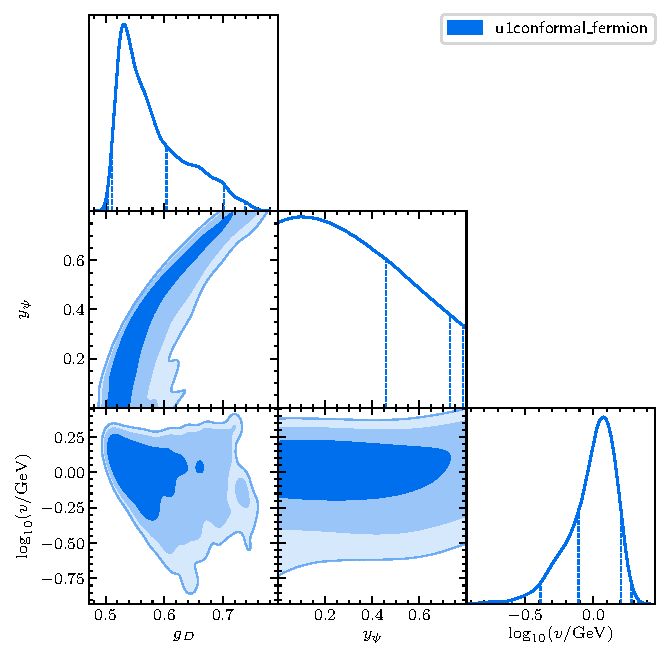
\includegraphics[width=0.9\textwidth]{u1conformal_fermion_posteriors.pdf}
\caption{Alternative posterior corner plot from the PTArcade analysis.}
\label{fig:posteriors_alt}
\end{figure}

%==================================================================
% References
%==================================================================

\newcommand{\arxiv}[1]{\href{https://arxiv.org/abs/#1}{arXiv:#1}}

\begin{thebibliography}{99}

\bibitem{Coleman:1973jx}
S.~R.~Coleman and E.~J.~Weinberg,
``Radiative Corrections as the Origin of Spontaneous Symmetry Breaking,''
Phys.\ Rev.\ D \textbf{7}, 1888--1910 (1973).
\arxiv{hep-th/0507214}

\bibitem{Khoze:2023}
V.~V.~Khoze and D.~L.~Milne,
``Gravitational waves and dark matter from classical scale invariance,''
Phys.\ Rev.\ D \textbf{107}, 095012 (2023).
\arxiv{2212.04784}

\bibitem{Balan:2025}
S.~Balan, T.~Bringmann, F.~Kahlhoefer, J.~Matuszak, and C.~Tasillo,
``Sub-GeV dark matter and nano-Hertz gravitational waves from a classically conformal dark sector,''
JCAP \textbf{08} (2025) 062.
\arxiv{2502.19478}

\bibitem{Goncalves:2025}
J.~Goncalves, D.~Marfatia, A.~P.~Morais, and R.~Pasechnik,
``Supercooled phase transitions in conformal dark sectors explain NANOGrav data,''
Phys.\ Lett.\ B \textbf{869}, 139829 (2025).
\arxiv{2501.11619}

\bibitem{Banik:2024}
A.~Banik, Y.~Cui, Y.-D.~Tsai, and Y.~Tsai,
``The Sound of Dark Sectors in Pulsar Timing Arrays,''
(2024).
\arxiv{2412.16282}

\bibitem{Borah:2021}
D.~Borah, A.~Dasgupta, and S.~K.~Kang,
``Gravitational waves from a dark U(1)$_D$ phase transition in the light of NANOGrav 12.5 yr data,''
Phys.\ Rev.\ D \textbf{104}, 063501 (2021).
\arxiv{2105.01007}

\bibitem{Costa:2025}
F.~Costa, J.~Hoefken Zink, M.~Lucente, S.~Pascoli, and S.~Rosauro-Alcaraz,
``Supercooled Dark Scalar Phase Transitions explanation of NANOGrav data,''
Phys.\ Lett.\ B \textbf{868}, 139634 (2025).
\arxiv{2501.15649}

\bibitem{Feng:2026}
W.-Z.~Feng and Z.-H.~Zhang,
``Gauge-independent gravitational waves from a minimal dark U(1) sector with viable dark matter candidates,''
(2026).
\arxiv{2602.14866}

\bibitem{Mahapatra:2026}
S.~Mahapatra, P.~K.~Paul, and N.~Sahu,
``Forbidden dark matter assisted by first-order phase transition and associated gravitational waves,''
(2026).
\arxiv{2601.12319}

\bibitem{Li:2026}
J.~Li and P.~Nath,
``Gravitational waves from supercooled phase transitions and pulsar timing array signals,''
Phys.\ Rev.\ D \textbf{111}, 123007 (2026).
\arxiv{2602.14324}

\bibitem{Ferrante:2023}
S.~Ferrante, A.~Ismail, S.~J.~Lee, and Y.~Lee,
``Forbidden conformal dark matter at a GeV,''
JHEP \textbf{11} (2023) 186.
\arxiv{2308.16219}

\bibitem{Fujikura:2023}
K.~Fujikura, Y.~Girmohanta, Y.~Nakai, and M.~Suzuki,
``NANOGrav Signal from a Dark Conformal Phase Transition,''
Phys.\ Lett.\ B \textbf{846}, 138203 (2023).
\arxiv{2306.17086}

\bibitem{Mohamadnejad:2020}
A.~Mohamadnejad,
``Gravitational waves from scale-invariant vector dark matter model: Probing below the neutrino-floor,''
Eur.\ Phys.\ J.\ C \textbf{80}, 553 (2020).
\arxiv{1907.08899}

\bibitem{Lewicki:2025}
M.~Lewicki and V.~Vaskonen,
``Dissipative bulk flow in strongly supercooled phase transitions,''
(2025).
\arxiv{2511.15687}

\bibitem{Mitridate:2023}
A.~Mitridate et al.,
``PTArcade,''
\url{https://github.com/mitridate/PTArcade}

\bibitem{Cline:2024}
J.~M.~Cline,
``Status of Dark Photons,''
(2024).
\arxiv{2405.08534}

\bibitem{Caputo:2025}
A.~Caputo, M.~Park, and S.~Yun,
``The Heavy Dark Photon Handbook,''
(2025).
\arxiv{2511.15785}

\bibitem{Giovanetti:2022}
C.~Giovanetti, M.~Lisanti, H.~Liu, and J.~T.~Ruderman,
``Joint CMB and BBN Constraints on Light Dark Sectors with Dark Radiation,''
Phys.\ Rev.\ Lett.\ \textbf{129}, 021302 (2022).
\arxiv{2109.03246}

\bibitem{Planck:2020}
Planck Collaboration,
``Planck 2018 results. VI. Cosmological parameters,''
Astron.\ Astrophys.\ \textbf{641}, A6 (2020).
\arxiv{1807.06209}

\bibitem{Araki:2024}
T.~Araki, K.~Asai, M.~Nakashima, and T.~Shimomura,
``Dark photon pair production via off-shell dark Higgs at FASER,''
(2024).
\arxiv{2406.17760}

\bibitem{Bogorad:2023}
Z.~Bogorad, P.~W.~Graham, and H.~Ramani,
``Coherent self-interactions of dark matter in the Bullet Cluster,''
(2023).
\arxiv{2311.07648}

\bibitem{Bai:2021}
Y.~Bai and M.~Korwar,
``Cosmological Constraints on First-Order Phase Transitions,''
(2021).
\arxiv{2109.14765}

\bibitem{Barman:2022}
B.~Barman, N.~Bernal, A.~Das, and A.~Racioppi,
``Gravitational production of dark matter during reheating,''
(2022).
\arxiv{2210.05716}

\bibitem{Deng:2023}
Z.~Deng and L.~Bian,
``Lower $N_{\rm eff}$ from strong first-order phase transitions,''
(2023).
\arxiv{2304.06576}

\bibitem{Christiansen:2025}
O.~Christiansen, M.~Niemi, J.~Rothkopf, and K.~Rummukainen,
``High-temperature effective theory for supercooled phase transitions,''
(2025).
\arxiv{2511.02910}

\bibitem{Camargo-Molina:2024}
J.~E.~Camargo-Molina, T.~V.~I.~Tennakone, and A.~W.~Weiler,
``Gauge dependence of the effective potential in the high-temperature expansion,''
(2024).
\arxiv{2410.23210}

\bibitem{Curtin:2018}
D.~Curtin, P.~Meade, and H.~Ramani,
``Thermal Resummation and Phase Transitions,''
(2018).
\arxiv{1808.08849}

\bibitem{Ellis:2018}
J.~Ellis, M.~Lewicki, and J.~M.~No,
``On the maximal strength of a first-order electroweak phase transition and its gravitational wave signal,''
JCAP \textbf{04} (2019) 003.
\arxiv{1809.08242}

\bibitem{Garcia:2022}
I.~Garcia Garcia, G.~Kosmo, and M.~Pieri,
``Bubble wall velocity in first-order phase transitions with massive gauge bosons,''
(2022).
\arxiv{2212.10572}

\bibitem{Kierkla:2023}
M.~Kierkla, A.~Karam, and B.~Swiezewska,
``Scalar contributions to the CW potential in conformal models,''
JHEP \textbf{01} (2024) 124.
\arxiv{2312.12413}

\bibitem{Pascoli:2026}
S.~Pascoli, J.~Hoefken Zink, and S.~Rosauro-Alcaraz,
``Renormalisation scale prescription for thermal phase transitions,''
(2026).
\arxiv{2602.02829}

\end{thebibliography}

\end{document}